%Grundlagen.tex

\section{Grundlagen}
\label{sec:Grundglagen}
\subsection{Ladung}
\label{sec:Ladung}
\[
Q=I\cdot t
\]
\[
[Q]=C=As
\]

\subsection{Stromdichte}
\label{sec:Stromdichte}
$ A $: Leiterquerschnitt
\[
J=\frac{I}{A}
\]
\[
[J] = \frac{A}{m^2}
\]
\subsection{Str�mungsgeschwindigkeit der Elektronen}
\label{sec:Str�mungsgeschwindigkeitDerElektronen}
$ v $: St�mungsgeschwindigkeit, $ e $: Elementarladung, $n$: Elektronendichte, $A$: Leiterquerschnitt
\[
v=\frac{I}{e\cdot n\cdot A}
\]

\subsection{Spannung}
\label{sec:Spannung}
\[
U=\frac{W}{Q}
\]
\[
[U]=V=\frac{Nm}{As}=\frac{kgm^2}{As^3}
\]

\subsection{Das ohmsche Gesetz (Widerstand)}
\label{sec:DasOhmscheGesetzWiderstand}
\[
R=\frac{U}{I}
\]
\[
[R]=\frac{V}{A}=\Omega
\]
\[
G=\frac{I}{U}=\frac{1}{R}
\]
\[
[G]=\frac{A}{V}=\frac{1}{R}
\]

\subsection{Spezifischer Widerstand}
\label{sec:SpezifischerWiderstand}
$\rho:$ spezifischer Widerstand, $l$: L�nge des Leiters, $A$: Querschnittsfl�che des Leiters
$\kappa$: spezifische Leitf�higkeit
\[
R=\frac{\rho\cdot l}{A}
\]
\[
[\rho]=\frac{\Omega m^2}{m}=\Omega m
\]
\[
\kappa=\frac{1}{\rho}
\]
\[
[\kappa]=\frac{1}{\Omega m}=\frac{S}{m}
\]
\[
R=\frac{l}{\kappa\cdot A}
\]
\subsection{Temperaturabh�nigkeit des Widerstandes}
\label{sec:Temperaturabh�nigkeitDesWiderstandes}
$R_1$: Widerstand bei $\vartheta_1$, $R_2$: Widerstand bei $\vartheta_2$, $\vartheta_1$: Ausgangstemperatur, $\vartheta_2$: Endtemperatur, $\alpha_1$: Temperaturkoeffizient
\[
R_2=R_1[1+\alpha_1(\vartheta_2-\vartheta_1)]
\]

\subsection{Leistung und Arbeit(Energie)}
\label{sec:ArbeitUndLeistung}
\[
P=U\cdot I=\frac{U^2}{R}=I^2\cdot R
\]
\[
[P]=W=VA=\frac{J}{s}=\frac{Nm}{s}=\frac{kg m^2}{s^3}
\]
\[
W=E=P\cdot t
\]
\[
[W]=[E]=J=Ws=VAs=Nm=\frac{kgm^2}{s^2}
\]

\subsection{Wirkungsgrad}
\label{sec:Wirkungsgrad}
$\eta: Wirkungsgrad$
\[
\eta=\frac{P_{ab}}{P_{zu}}
\]
%\subsection{Pfeilsysteme}
%\label{sec:Pfeilsysteme}

\subsection{Umwandlung von Quellen}
\label{sec:UmwandlungVonQuellen}


\begin{figure}[H]
	\centering
%		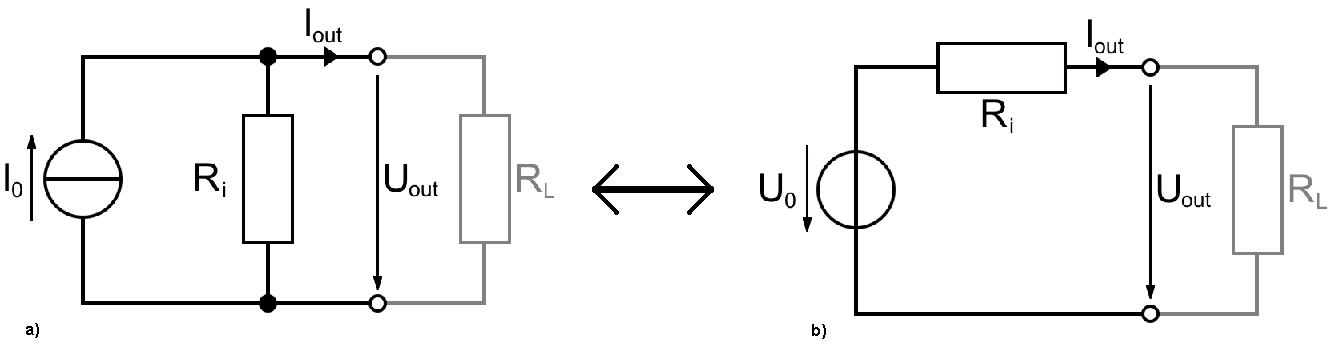
\includegraphics[width=8CM]{Grafiken/reale_Quellen.png}	
	\caption{reale Quellen mit Innenwiderstand}
	\label{fig:reale_Quellen}
\end{figure}


Bei der Umwandlung von Quellen zeigt der Pfeil der neuen Quelle entgegengesetzt der vorherigen Quelle. Siehe Abbildung \ref{fig:reale_Quellen} Seite \pageref{fig:reale_Quellen}

\paragraph{Stromquelle $\rightarrow$ Spannungsquelle}
\label{sec:StromquelleSpannungsquelle}
\[
U_q=I_q\cdot R_i
\]

\paragraph{Spannungsquelle $\rightarrow$ Stromquelle}
\label{sec:SpannungsquelleStromquelle}
\[
I_q=\frac{U_q}{R_i}
\]



\subsection{Die Kirchhoff'schen Gesetze}
\label{sec:DieKirchhoffSchenGesetze}

\subsubsection{Knotenregel}
\label{sec:Knotenregel (1. Kirchhoff'sches Gesetz}
Die Summe aller Str�me die in einen Knotenpunkt f�hren ist Null.
\[
\sum_{k=1}^nI_k = 0
\]

%(Bild)

\subsubsection{Maschenregel (2. Kirchhoff'sches Gesetz)}
\label{sec:Maschenregel}
Die Summe aller Spannungen in einer Masche ist Null.
\[
\sum_{k=1}^nU_k = 0
\]
%(Bild)

